%%%%%%%%%%%%%%%%%%%%%%%%%%%%%%%%%%%%%%%%%%%%%%%%%%%%%%%%%%%%%%%%%%%%%%%%%%%%%%%%
%2345678901234567890123456789012345678901234567890123456789012345678901234567890
%        1         2         3         4         5         6         7         8

\documentclass[letterpaper, 10 pt, conference]{ieeeconf}  % Comment this line out
                                                          % if you need a4paper
%\documentclass[a4paper, 10pt, conference]{ieeeconf}      % Use this line for a4
                                                          % paper

\IEEEoverridecommandlockouts                              % This command is only
                                                          % needed if you want to
                                                          % use the \thanks command
\overrideIEEEmargins
% See the \addtolength command later in the file to balance the column lengths
% on the last page of the document



% The following packages can be found on http:\\www.ctan.org
\usepackage{graphics} % for pdf, bitmapped graphics files
\usepackage{epsfig} % for postscript graphics files
%\usepackage{mathptmx} % assumes new font selection scheme installed
%\usepackage{times} % assumes new font selection scheme installed
\usepackage{amsmath} % assumes amsmath package installed
%\usepackage{amssymb}  % assumes amsmath package installed
%\usepackage[style=numeric-comp]{biblatex}
%\usepackage[numbers,sort&compress]{natbib}
\usepackage[compress]{cite}
\usepackage[utf8]{inputenc}
\usepackage[T1]{fontenc}


\title{\LARGE \bf
Humanoid Throwing: Design of Collision-Free Trajectories with Sparse Reachable Maps
}

%\author{ \parbox{3 in}{\centering Huibert Kwakernaak*
%         \thanks{*Use the $\backslash$thanks command to put information here}\\
%         Faculty of Electrical Engineering, Mathematics and Computer Science\\
%         University of Twente\\
%         7500 AE Enschede, The Netherlands\\
%         {\tt\small h.kwakernaak@autsubmit.com}}
%         \hspace*{ 0.5 in}
%         \parbox{3 in}{ \centering Pradeep Misra**
%         \thanks{**The footnote marks may be inserted manually}\\
%        Department of Electrical Engineering \\
%         Wright State University\\
%         Dayton, OH 45435, USA\\
%         {\tt\small pmisra@cs.wright.edu}}
%}

\author{Daniel M. Lofaro$^{1}$, Robert Ellenberg$^{2}$, Paul Oh$^{2}$, and Jun-Ho Oh$^{3}$\\
Electrical Engineering$^1$ and Mechanical Engineering$^2$ Dept., Drexel University, Philadelphia PA, USA\\
Mechanical Engineering$^3$ Dept., Korean Advanced Institute of Science and Technology, Daejeon, S. Korea\\
\ttfamily{dml46@drexel.edu, rwe24@drexel.edu, paul@coe.drexel.edu, jhoh@kaist.ac.kr}% <-this % stops a space
\thanks{*This project was supported by a Partnerships for International Research and Education (PIRE) grant \#0730206, sponsored by the the U.S. National Science Foundation (NSF)}% <-this % stops a space
}
%\thanks{$^{1}$D. Lofaro is a Ph.D Candidate with the Electrical Engineering Department, Drexel University, Philadelphia PA, USA
%        {\tt\small dan at danlofaro.com}}%
%\thanks{$^{2}$R. Ellenberg is a Ph.D Candidate with the Mechanical Engineering Department, Drexel University, Philadelphia PA, USA
%        {\tt\small rwe24 at drexel.edu}}%
%\thanks{$^{3}$J. Oh is faculty with the Department of Mechanical Engineering, Korean Advanced Institute of Science and Technology, Daejeon, S. Korea
%        {\tt\small jhoh at kaist.ac.kr}}%
%\thanks{$^{4}$P. Oh is faculty with the Department of Mechanical Engineering, Drexel University, Philadelphia PA, USA
%        {\tt\small paul at coe.drexel.edu}}%
%}


\begin{document}



\maketitle
\begin{center}
\end{center}
\thispagestyle{empty}
\pagestyle{empty}



%%%%%%%%%%%%%%%%%%%%%%%%%%%%%%%%%%%%%%%%%%%%%%%%%%%%%%%%%%%%%%%%%%%%%%%%%%%%%%%%
\begin{abstract}
	\begin{center}
\large\bf{Abstract:}
\end{center}
\normalsize

\bf{
\noindent The degrees of freedom (DOF) of robots and complex systems have been increasing increasing exponentially since the early 20th century.
Today it is common place for complex control systems to have 40 DOF. 
This number is projected to be 70 DOF by the year 2020.
Robots with high DOF allows for complex tasks such as tool manipulation, greater human-robot interaction and agile full-body locomotion.
More DOF require greater attention to local communication delays, bandwidth, system configuration and stability.
In addition different tasks being performed by separate parts of the robot in tandem bring on greater issues including controller timing and priorities.
The increase in DOF on single system requires that the traditional methods of controller design be re-examined.

\noindent This dissertation describes a Unified Algorithmic Framework for High Degree of Freedom Complex Systems and Humanoid Robots that allows a user to develop controllers using a three tier infrastructure.
The Unified Algorithmic Framework called Hubo-Ach is a multi-process based system that allows for robust multi-rate simultaneous control and seamless implementation between virtual, miniature, and full-size robots with no modification.
The three tier infrastructure provides different levels of cost to entry and testing.
Examples of this field tested framework functioning on simulated, miniature, and full-size high DOF robots is given as well as validation by external researchers.
}




\end{abstract}


%%%%%%%%%%%%%%%%%%%%%%%%%%%%%%%%%%%%%%%%%%%%%%%%%%%%%%%%%%%%%%%%%%%%%%%%%%%%%%%%
%\section{INTRODUCTION}
	The number of degrees of freedom (DOF) of control systems are increasing exponentially since the early 20$^{th}$ century.
Today it is common place for complex control systems to have 40 DOF. 
This number is projected to be 70 DOF by the year 2020 (see Section~\ref{sec:numdof}).
\textit{The increase in DOF on single system requires that the traditional methods of controller design needs to be re-examined}.
High DOF complex system, or robots, allow for complex tasks such as using human tools and interfaces \cite{lofaroRAM2013,lofaroTePRA2013HuboAch,lofaroTePRA2013Valve,gtechIK}, playing music \cite{lofaroEURASIP2011, 6094987,lofaroIASTED2011,5686847} and other complex tasks \cite{lofaroHumanoids2012,lofaroGamesRobot,tepraLadder2013}.

\cite{orocos-gadeyne-ijrr2005}
\cite{multiPC-arch-1185243}
\cite{multi-thread-robot-5602743}
\cite{multi-thread-snake-1541141}
\cite{multi-thread-5524083}
\cite{openHRP}
\cite{Webots}




Due to the nature of these highly redundant complex electrical mechanical system it is common to have multiple different controllers running in tandem.  
Different controllers are needed when the system is in different states or doing different tasks or performing multiple tasks at the same time.
Combining these controllers is a problem in complex system.
This problem is hard when each controller has different frequencies, timing requirements (asyncronous vs. syncronous), latency restrictions, newest state data ie smore important then older state data and most basic of all languages the controller is written in.
This is especially true for complete and complex autonomous systems.
I define a complete and complex autonomous system as an electro mechanical mechanism with high degree of freedom (DOF) that is capable of making its own decisions through the use of sensor data processed by its artificial intelligence (AI).
The combination of high DOF and the requirement for autonomy makes the work space broad and controllers complex.
The overarching question becomes; What is the control system structure for a complete and complex autonomous systems with high DOF, a multitude of sensors, AI performing high-level and low-level tasks all while keeping a stable system structure conducive to collaborative work?
Current methods of solving the problem of controller synchrony and latest state data is to keep your critical control elements in the primary control loop.
Inter-process communication (IPC) and/or network sockets to communicate between the high level and low level processes even if written in different languages.
The majority of IPC have the problem of \textit{head of line} blocking (HOL) which means you must read the older data in a buffer before you read the newest data.
In the computer science field this is not a problem because all data being intact is typically desired.  
In the field of robotics and control the most recent state data is more important to a real-time control system to act on.
This thesis shows that by expanding on the idea of multi-process controllers connected to high-speed low-latency IPC you can create a \textit{robot layer} on a computer platform that will allow low-level controllers to run in separate processes while still allowing them access to the most recent data as the priority.
The new technical idea is the \textit{robot layer}, a control layer that allows external processes to run like normal and not deal with the specifics of the given robot system.
The robot system can be replaced by a simulated system without any of the processes needing to be modified or even know of the change.
This allows more mature controllers to be easily interfaced with this system without modifying control rates or timing.
This \textit{robot layer} must be:
\begin{itemize}
\item Have a IPC latency much less then that of the robot's inherent sampling period $t_{ipc}<<T_{r}$
\item Allow for command rates much slower then the inherent sampling period $T_{slow}>>T_{r}$
\item Allow for command rates much faster then the inherent sampling period $T_{fast}<<T_{r}$
\item Allow for arbitrary command rates.
\item Allow for real-time and non-real-time controllers to command actuators
\item Allow for all processes to have access to the newest data first
\item Allow for no more then one rt time step delay between command and robot actuator retrieval
\item Commanded such that it is for an arbitrary robotic actuator.
\item Triggering for process synchronization
\item Triggering for simulator synchronization and holding
\end{itemize}
We can succeed now not only because the bleeding edge technology allows for the fast enough communication between processes with access to the latest data.

Results are measured quantitatively and qualitatively.
Data showing proper loop rates, timings, controller implementation, simulation connections etc. show the viability of the system.
User survey shows methodology is sound, useful, and practical.





My Thesis shows is that a multi-process control structure coupled with the proper timing mechanisms is conducive to answering these questions.
It is shown with physical experiments and the creation of Hubo-Ach\cite{lofaroRAM2013}; a fully functional Sim-Time and Real-Time control system for complete and complex autonomous systems.

Through experimentation I prove my control system is a viable way of controlling complete and complex autonomous system and still be conducive to collaborative work.  
A road map of how my research has taken me to my thesis is shown in Section~\ref{sec:roadmap}.
As proof of viability I show the basic structure of my system \textit{Hubo-Ach} in Section~\ref{sec:hubo-ach}.  
I give step by step examples in Section~\ref{sec:simpleExamples}.
Section~\ref{sec:simulator} shows how we can move from real-time to using a simulated version of the platform in simulation time without having to change the controller.
Section~\ref{sec:task} describes the experiment which consists of making the robot preform an advanced task that pulls together visual, kinematic, path planning and other controllers together using this one system.
The techniques used stem from my contributions in Section~\ref{sec:contributions}.
Section~\ref{sec:results} shows the results of the experiment thus show the viability of the system.
Lastly Section~\ref{sec:conclusion} discusses the results of the work and the future of this system.

Before I continue it is important to note that my work has already been validated by my pears because:
\begin{itemize}
\item It was chosen to be the primary control system for the DARPA Robotics Challenge Track-A Team DRC-Hubo, Section~\ref{sec:drc}.
\item It is being used in the NSF-MIRR project\footnote{NSF-MIRR: Major Research Infrastructure Recovery and Reinvestment (MIRR) \#CNS-0960061 sponsored by the the U.S. National Science Foundation (NSF)}.
\item It is currently being used by MIT, WPI, Purdue, Ohio State, Swarthmore College, Georgia Tech, and Drexel University.
\end{itemize}

For the remainder of this document the complete and complex autonomous systems that I will be referring to are robots.
The majority of examples given will be in reference to humanoid robotics and the Hubo2+ (KHR-4+) platform.
The Hubo platform is described in Section~\ref{sec:hubo}.





	
% \section{RELATED WORK}
%	\section{RELATED WORK}

Low degree of freedom throwing machines/robots are common.  
%Typical throwing robots have between one and three degrees of freedom (DOF) \cite{509405,Lynch97dynamicnonprehensile,5152525,509335,springerlink:10.1007/s10015-006-0401-0}.  
All of these mechanisms are limited to throwing in a plane.   
Sentoo et al.\cite{4651142} achieved an end-effector velocity of 6.0 m/s and can throw in $R^3$ space using it's Barret Technology Inc 4-DOF arm with a $360^o$ rotation base yaw actuator.  
These low degree of freedom throwing robots are either physically attached/planted to the mechanical ground or have a base that is significantly more massive then the arm.  

%\cite{5686315,JooH2011438}
Kim et al. \cite{JooH2011438} takes the research to the next level with finding optimal overarm and sidearm throwing motions for a high degree of freedom humanoid computer model.  
The model consists of 55-DOF and is not fixed to mechanical ground or a massive base.  
Motor torques are then calculated that both allows for a sidearm or overarm throw and continuously satisfies the zero-moment-point stability criteria \cite{4309277}.  

%Kim was able to receive a maximum flight time of 2.784s and 3.711s for overarm and sidearm throws respectively.



	
	
% \section{METHODOLOGY}
	\section{Methodology}\label{sec:methodology}
%\subsection{Balance and Stability}\label{sec:sec:balance}
Each of the methods used have to be stable through the motion in order for the system to be stable (i.e. not to fall down).  
The well known zero-moment-point (ZMP) criteria is what each method must adhere to in order to stay statically stable\cite{Vukobratovic19721}.  
To handle perturbation an active balance controller was added.  
The active balance controller is applied on top of the pre-defined trajectories.  
Hubo is modeled as a single inverted pendulum with the center of mass (COM) located at length $L$ from the ankle.  
The compliance of the robot is composed of a spring $K$ and a damper $C$, see Fig.~\ref{fig:invPen}.  
An IMU located at the COM gives the measured orientation.

\begin{figure}[t]
  \centering
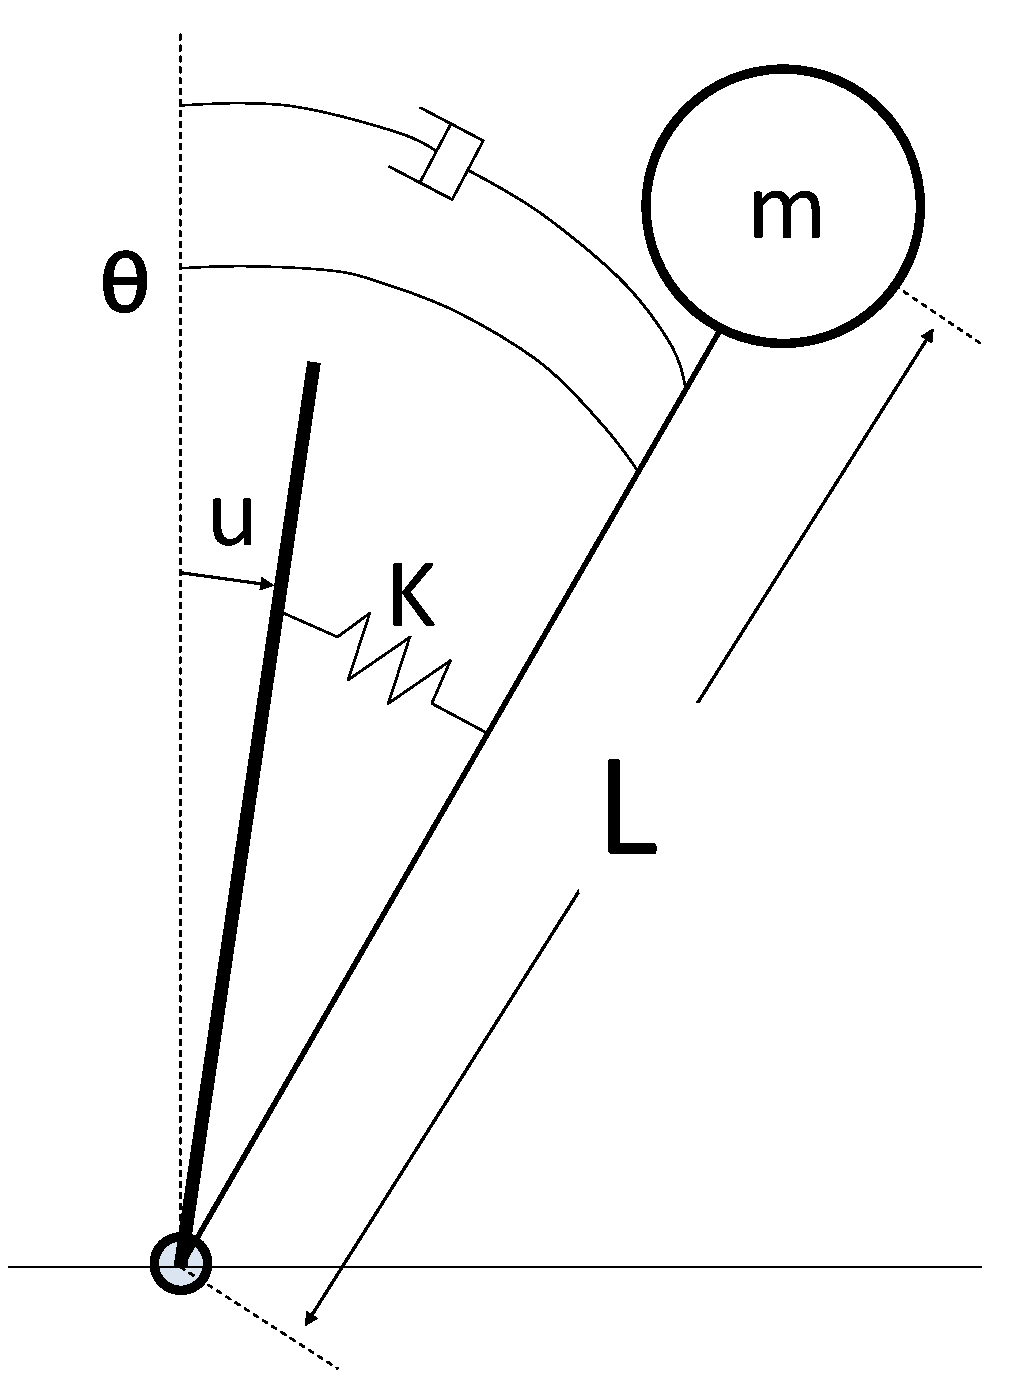
\includegraphics[width=0.4\columnwidth]{./pix/invPen3.pdf}
  \caption{Hubo modeled as a single inverted pendulum with COM located a distance $L$ from }
  \label{fig:invPen}
\end{figure}

The dynamic equation of the simplified model is assumed to be the same in both the sagittal and coronal plane.

\begin{equation}
mL^2\ddot{\theta}+C\dot{\theta}-K\theta = Ku
\end{equation}

This can be linearized and made into the transfer function:

\begin{equation}
%G(s) = \frac{\Theta(s)}{U(s)} = \frac{K}{ mL^2s^2 + Cs + (K - mgL)}
G(s) = \frac{\Theta(s)}{U(s)} = \frac{\frac{K}{mL^2}}{s^2+\frac{C}{mL^2}s + \frac{K-mgL}{mL^2}}
\end{equation}

Prior work on the model and controller for the Hubo by Cho et. al. calculated K=753 $\frac{Nm}{rad}$ and C=18 $\frac{Nm}{sec}$ using the free vibration response method\cite{5379574}.


\begin{figure}[ht]
  \centering
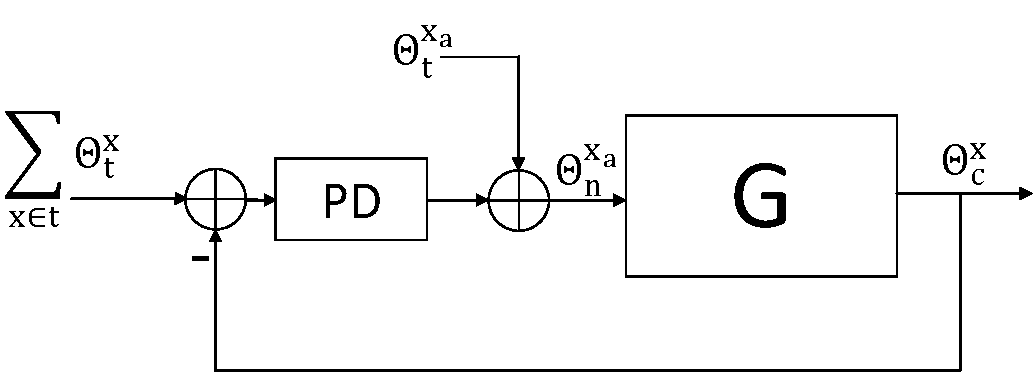
\includegraphics[width=0.8\columnwidth]{./pix/blockDiagram3.pdf}
  \caption{Block diagram of the balance controller used to balance Hubo in this work.}
  \label{fig:ctrlBlockDiagram}
\end{figure}

The control law is as follows
%ffFor the ankle roll (in the coronal plane) it is always assumed that the desired orientation of the COM is zero degrees.  Thus the roll of the IMU is taken as the error.

\begin{equation}
\theta_n^{x_a} = \theta_t^{x_a} + \left(K_p^x+sK_d^x\right)\left(\sum\limits_{x \in t} \theta_{t}^x - \theta_{c}^x\right)
%\theta_{n}^x = \theta_{t}^x + \left(K_p^x+sK_d^x\right)\left(\sum \theta_{t}^x - \theta_{c}^x\right)
%\theta_{n}^x = \theta_{t}^x + (K_p^x+sK_d^x)(\sum \theta_{t}^x - \theta_{c}^x)
%\theta_{new} = \theta_{traj} + (K_p+sK_d)(\sum \theta_{leg} - \theta_{IMU})
\end{equation}

Where $\theta_t$ is the desired trajectory of the lower body (pitch or roll), $x$ denotes pitch or roll and $x_a$ denotes pitch or roll on the ankle.  $\theta_{c}$ is the orientation of the center of mass in the global frame.  $\theta_n$ is the resulting trajectory.  $K_p$ and $K_d$ are the proportional and derivative gains.  The resulting control allows for a stable stance even with perturbations from upper body motions.




%\section{EXPERIMENT}
	\section{EXPERIMENT}\label{sec:exp}
The goal of throwing a projectile was set to 3.0 $m$, the maximum usable distance in the SISTR system as described Ellenberg et al.~\cite{5686325}.  The target is placed directly in front of the robot.  Using the SRM the release point for the projectile motion calculations was set to the mean of the right arm's reachable area, 0.8m from the ground in $z$.  This resulted in a throwing velocity of 4.9 $\frac{m}{s}$ at $[\Theta, \Psi, \Phi] =[0.0^o,45.0^o, 3.8^o]$.  This velocity was required to be sustained for 0.1 $sec$ due to the speed and accuracy of the gripper's release.  This velocity duration and direction forced the trajectory to produce an underhand throwing gesture.  The projectile is a standard racquetball measuring 57 $mm$ in diameter and weighting 42.7 $g$.  The light weight racquetball ball was chosen to assist in not causing instability.  $\vec{L}_d$ and the setup trajectory are created using the method shown in Section~\ref{sec:methodology} and following all specified constraints.  Fig.~\ref{fig:sparseRegion} shows $\vec{L}_d$ and the setup trajectory plotted within the SRM.

%\begin{figure}[thpb]
%  \centering
%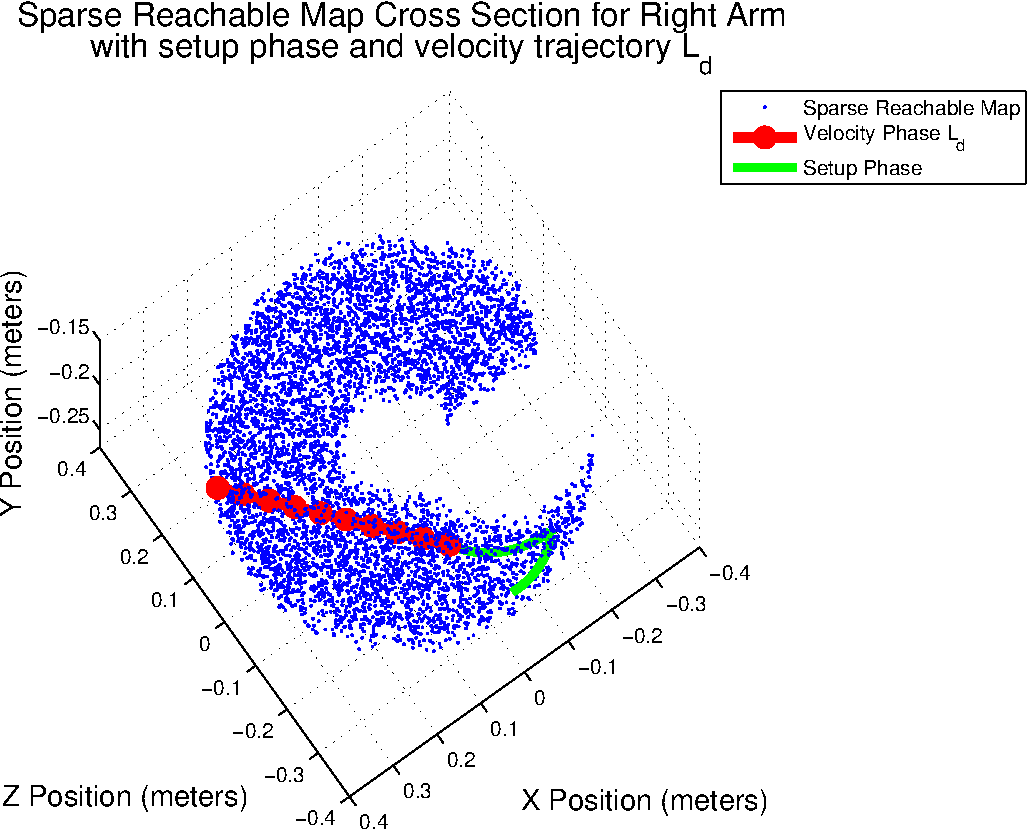
\includegraphics[width=1.0\columnwidth]{./MATLAB/throwTraj3D.pdf}
%  \caption{Sparse Reachable Map Cross Section for Right Arm with setup phase and velocity trajectory $L_d$ }
%  \label{fig:3dThrowPlot1}
%\end{figure}


\begin{figure}[thpb]
  \centering
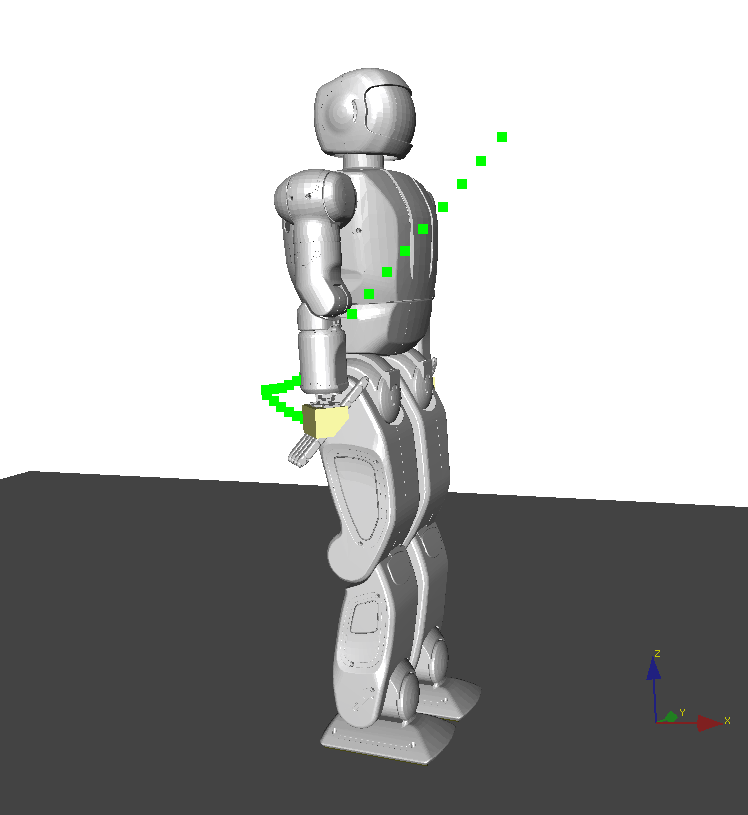
\includegraphics[width=0.25\columnwidth]{./pictures/ddFinal/vHside1.png}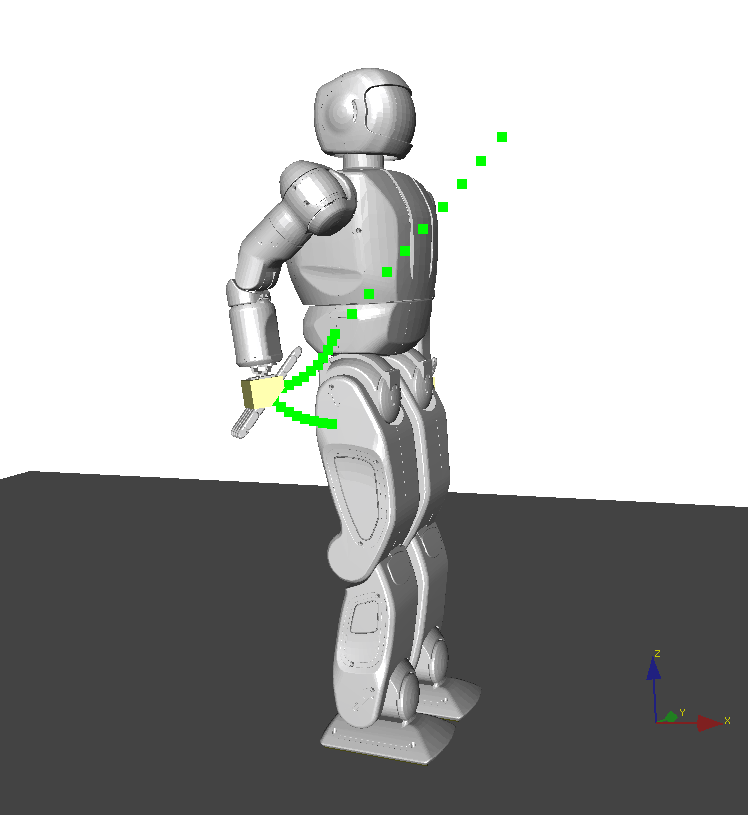
\includegraphics[width=0.25\columnwidth]{./pictures/ddFinal/vHside3.png}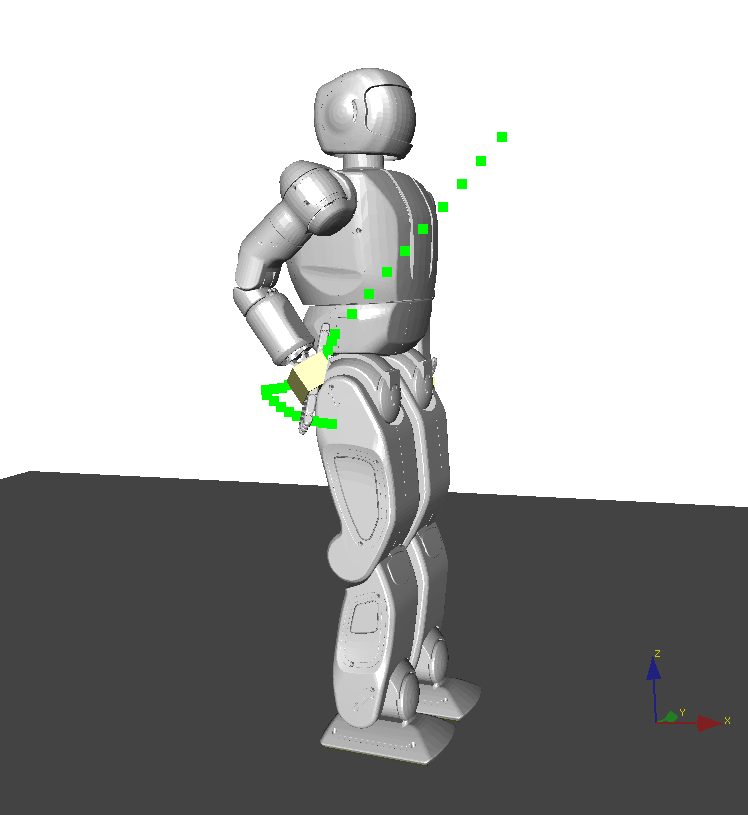
\includegraphics[width=0.25\columnwidth]{./pictures/ddFinal/vHside4.png}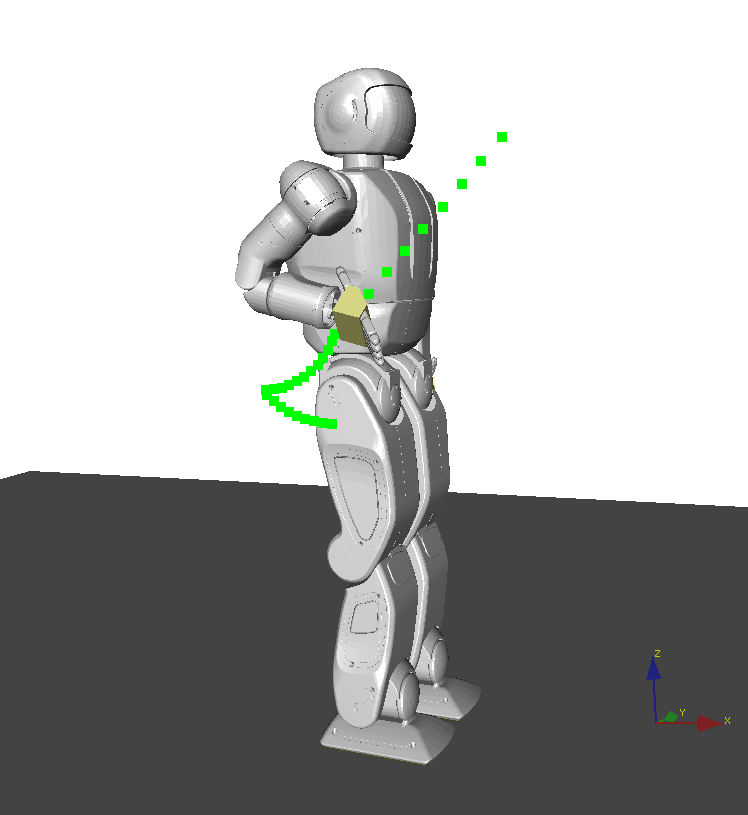
\includegraphics[width=0.25\columnwidth]{./pictures/ddFinal/vHside5.png}
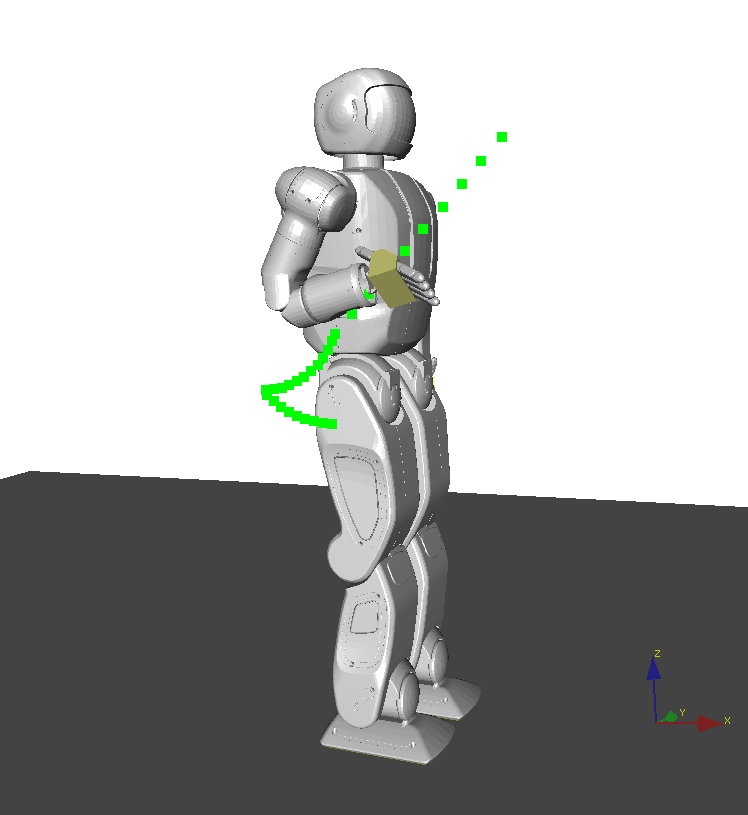
\includegraphics[width=0.25\columnwidth]{./pictures/ddFinal/vHside6.png}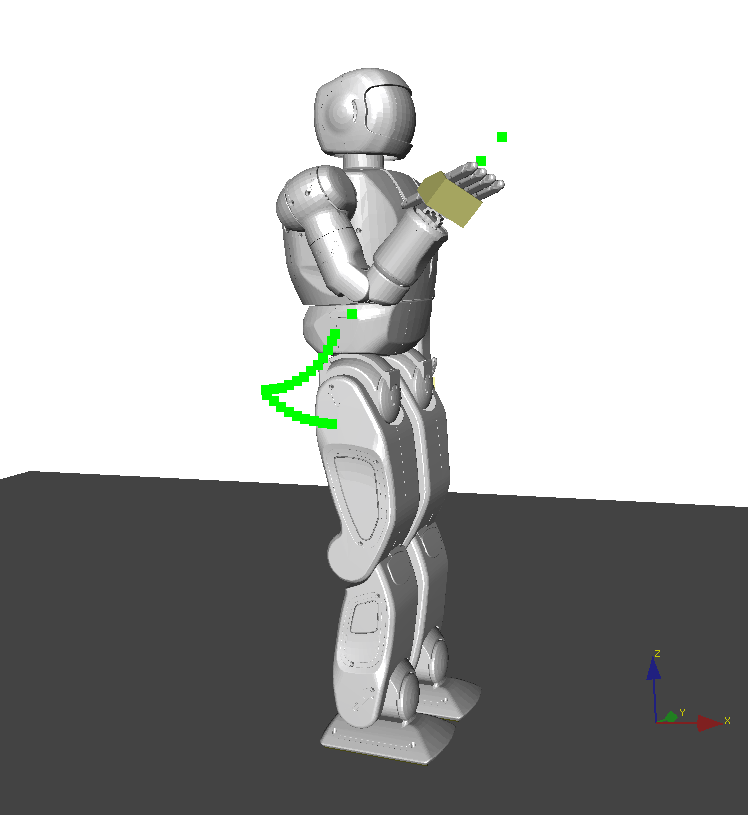
\includegraphics[width=0.25\columnwidth]{./pictures/ddFinal/vHside7.png}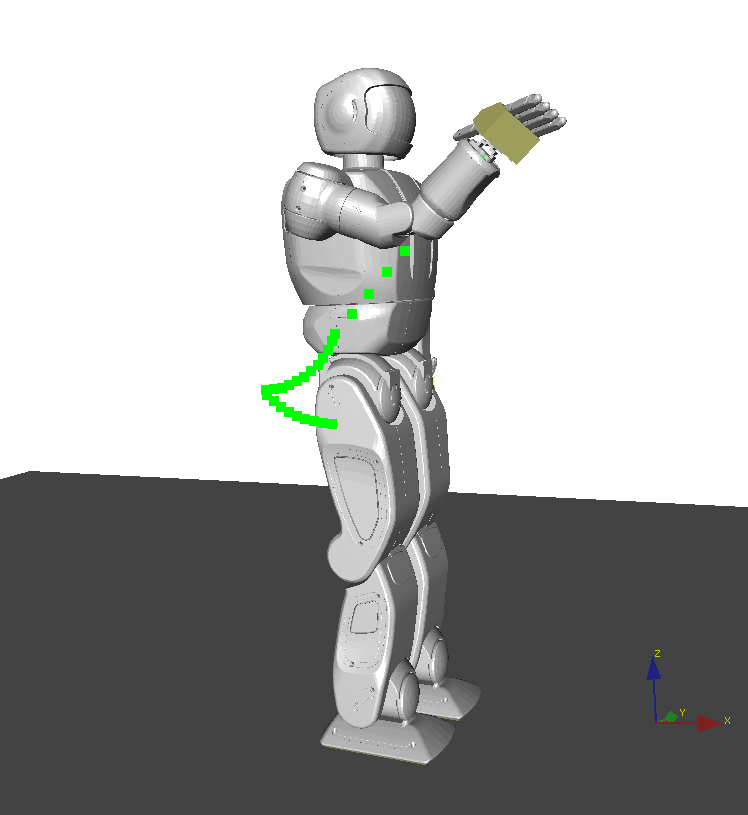
\includegraphics[width=0.25\columnwidth]{./pictures/ddFinal/vHside9.png}
  \caption{Jaemi Hubo running throwing trajectory $\vec{L}_d$ immediately after the setup phase is completed.  $\vec{L}_d(0)$ is top left.  Frames are read left to right and have a $\Delta t$ of 0.15 $sec$}
  \label{fig:fThrow}
\end{figure}



The trajectory was run on Jaemi Hubo with a position command period $T_r$ of 0.01 $sec$.  Fig~\ref{fig:3dThrowReal} shows the side profile of the Jaemi Hubo successfully running the trajectory.  The trajectory shown in Fig~\ref{fig:3dThrowReal} is considered an underhand throw, overhand and sidearm throws are also created with this method.

\begin{figure}[thpb]
  \centering
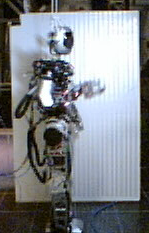
\includegraphics[width=0.25\columnwidth]{./pictures/slowMotion/1.png}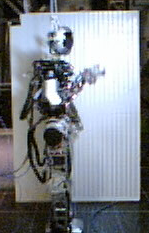
\includegraphics[width=0.25\columnwidth]{./pictures/slowMotion/2.png}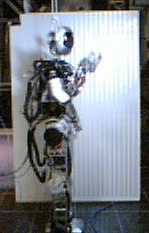
\includegraphics[width=0.25\columnwidth]{./pictures/slowMotion/3.png}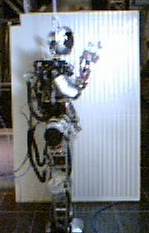
\includegraphics[width=0.25\columnwidth]{./pictures/slowMotion/4.png}
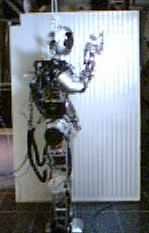
\includegraphics[width=0.25\columnwidth]{./pictures/slowMotion/5.png}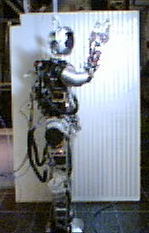
\includegraphics[width=0.25\columnwidth]{./pictures/slowMotion/6.png}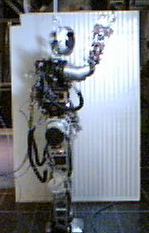
\includegraphics[width=0.25\columnwidth]{./pictures/slowMotion/7.png}
  \caption{Jaemi Hubo running throwing trajectory $\vec{L}_d$ immediately after the setup phase is completed.  $\vec{L}_d(0)$ is top left.  Frames are read left to right and have a $\Delta t$ of 0.15 $sec$}
  \label{fig:3dThrowReal}
\end{figure}

During the experiments the actual position of each joint was recorded.  The total time from the start of the setup phase to the end of the velocity phase is 0.31 $sec$.



%\section{EXPERIMENT \& RESULTS}
%\section{RESULTS}
	\section{RESULTS}\label{sec:reslts}
The system successfully generated and ran valid trajectories.  The commanded trajectory produces the desired velocity of 4.9 $\frac{m}{s}$.  The joint position of the physical joints were logged during run-time.  
The logged and commanded trajectories are seen plotted over the SRM in Fig.~\ref{fig:sparseRegion}.  
%The velocity and acceleration of the end-effector for the logged and commanded trajectories in the velocity phase can be seen Fig~\ref{fig:posPlot}.
%The end effector had large accelerations present when run on the physical system.  

%\begin{figure}[thpb]
%  \centering
%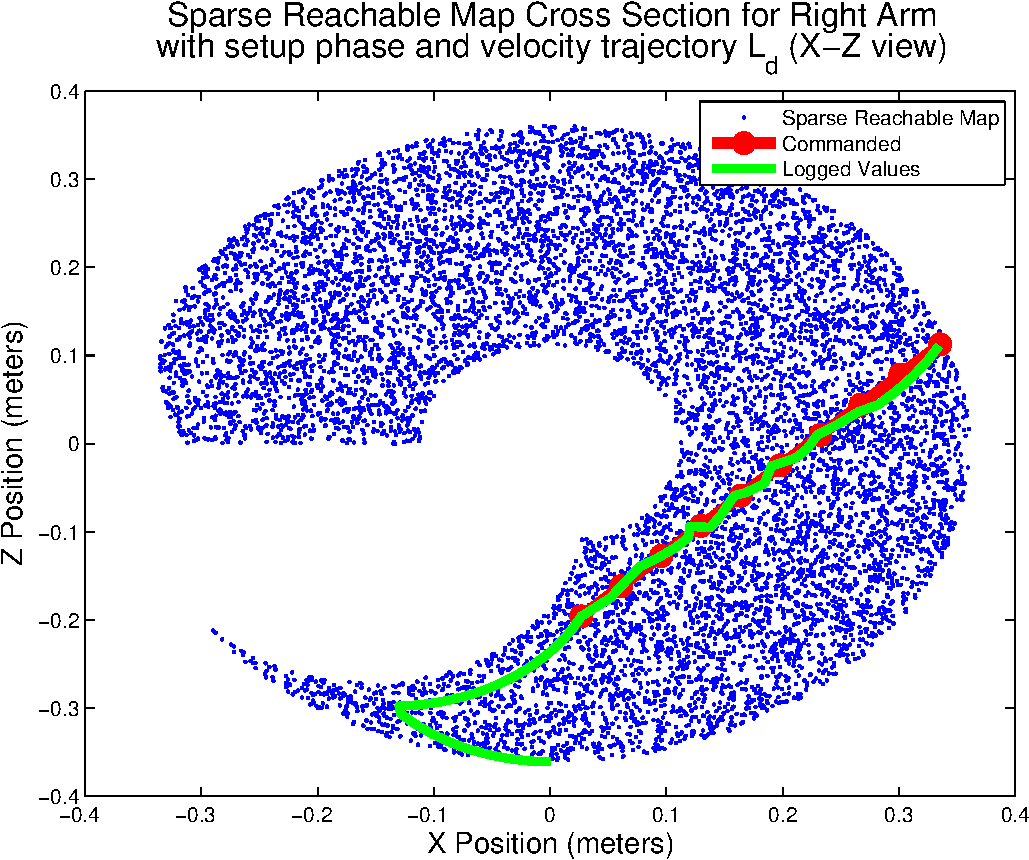
\includegraphics[width=1.0\columnwidth]{./MATLAB/throwTrajAct.pdf}
%  \caption{Commanded right arm end-effector position in $R^3$ from Fig.~\ref{fig:3dThrowPlot1} (red) and the logged joint space values converted to %$R^3$ using forward kinematics (green) shown over the sparse reachable map (blue).}
%  \label{fig:svmMap}
%\end{figure}

\begin{figure}[thpb]
  \centering
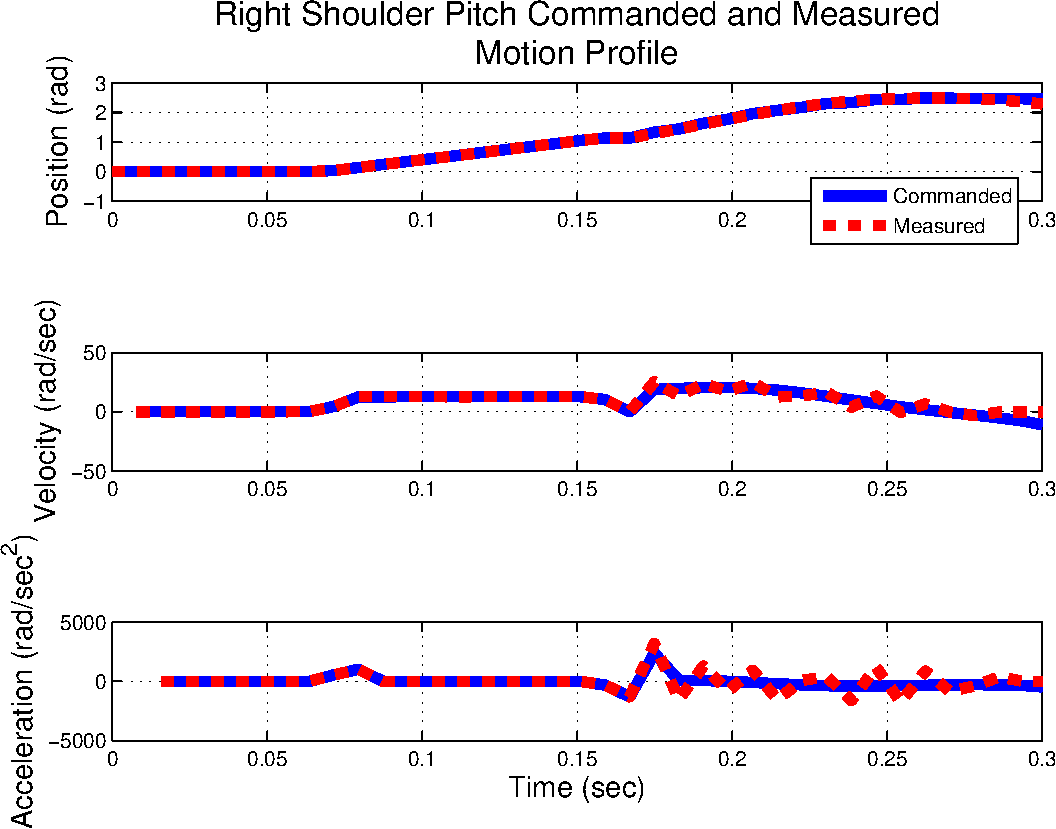
\includegraphics[width=1.0\columnwidth]{./MATLAB/throwTrajRSPplot.pdf}
  \caption{Right shoulder pitch commanded and measured motion profile; Position (top), Velocity (middle), Acceleration (bottom).  This is the result of running the trajectory shown in Fig.~\ref{fig:fThrow} and Fig.~\ref{fig:3dThrowReal}}
  \label{fig:velosPlot}
\end{figure}


The end-effector has large accelerations present in the physical system because some of the actuators are commanded with accelerations and torques beyond the capabilities of the physical actuator.  The angular velocity and acceleration of the right shoulder pitch joint can be seen in Fig.~\ref{fig:velosPlot}.  The large accelerations combined with the inertia of the arm caused the joint to overshoot the commanded position.  This caused over-torque on the pitch joint causing the joint to shutdown in slightly less then 10\% of the trials.



%\begin{figure}[thpb]
%  \centering
%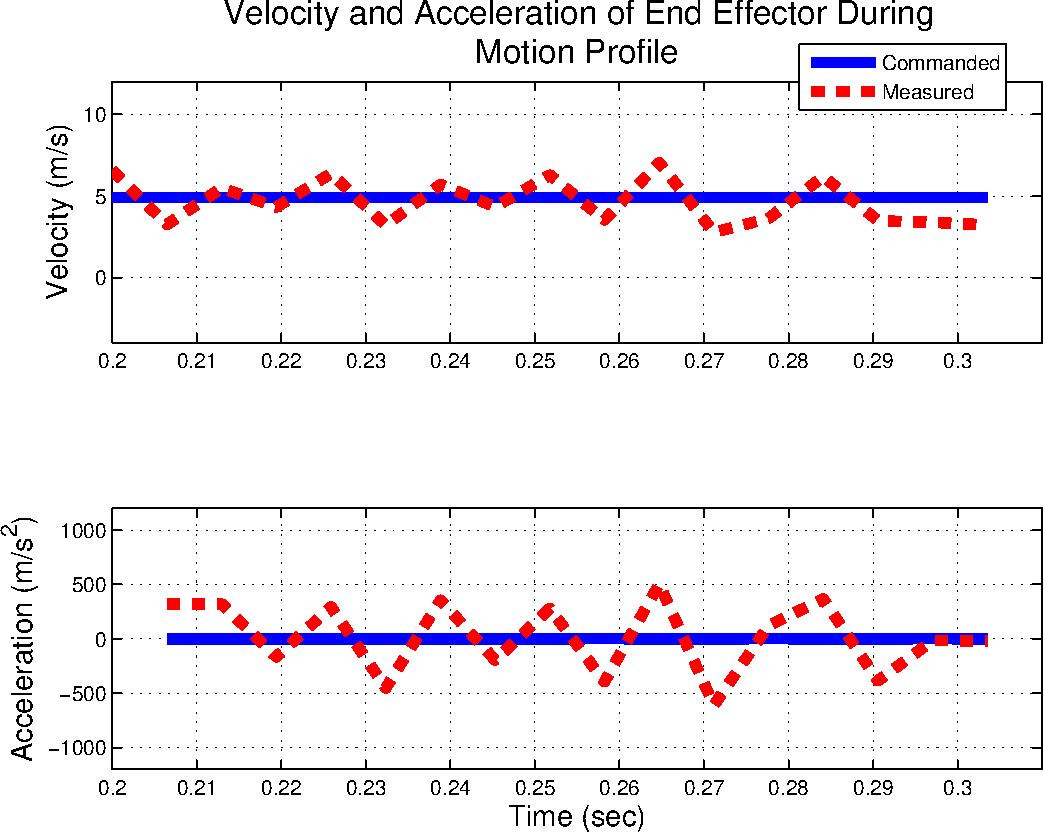
\includegraphics[width=1.0\columnwidth]{./MATLAB/throwTrajRSPacc.pdf}
%  \caption{The velocity and acceleration of the end-effector for the commanded trajectory and the recorded runtime log in the velocity phase; Velocity (top), Acceleration (bottom).  The is the result of running the trajectory shown in Fig.~\ref{fig:fThrow} and Fig.~\ref{fig:3dThrowReal}.}
%  \label{fig:posPlot}
%\end{figure}










%\section{CONCLUSION \& FUTURE WORK}
%\section{CONCLUSION}
	\section{CONCLUSION AND FUTURE WORK}\label{sec:conc}

As the results in Fig.~\ref{fig:sparseRegion} in Section~\ref{sec:reslts} show the approach presented in this paper was successful for underhand throwing.  This approach also preforms overhand throwing if the velocity direction, duration, and magnitude falls within the SRM.  While not presented in this paper, results of overhand throwing will be presented in future dissemination of this work.  This work is also constructed in such a way that it is easily applicable to other low and high DOF robots.

The paper described a solution that coincides with our future efforts.  The next logical step is to incorporate full body motion and balancing to the velocity trajectory calculations to further advance the overarching goal of full body end-effector velocity control.

%In the end we solved the problem in the direction that we are going in.  The next logical step is to incorporate full body motion and balancing to the velocity trajectory calculations to further advance us towards our overarching goal.


%This work has shown a valid method of creating trajectories to achieve end-effector velocity control for high degree of freedom position controlled robots.  It was shown the full reachable area does not need to be known to achieve the desired velocity if a good collision model of the robot is available.  It was found that the limiting factor was the robot's physical joints.  This system does create trajectories that fall within the actuators' limitations, however this is not guaranteed.  Immediate future work includes creating a system that will guarantee actuator compliance with the generated trajectory.
	
%\section{FUTURE WORK}
%	\input{futurework}

%\section{ACKNOWLEDGMENTS}
%	write something funny

%\cite{tempo}
\bibliographystyle{IEEEtran}
%\bibliographystyle{plain}
\bibliography{throwing}{}




\end{document}
